\documentclass[crop=false,fleqn]{standalone}
\usepackage{../../../globle-preamble}

\begin{document}
    \textbf{Express the area $A$ of circle as function of its circumference $C$.}

    \begin{center}
        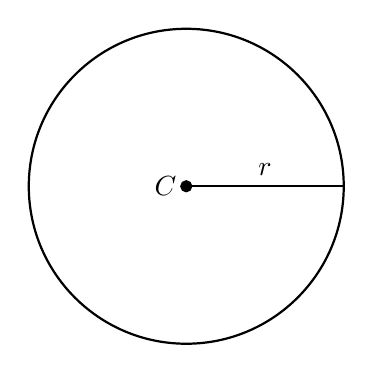
\begin{tikzpicture}
            \draw[thick] (0,0) circle (2);
            \draw[thick] (0,0) -- node[above]{$r$} (2,0);
            \filldraw (0,0) node[left]{$C$} circle (2pt);
        \end{tikzpicture}
    \end{center}

    Let,

    \begin{align*}
        \text{Area of a circle} = A &= \pi r^2 \\
        \text{Circumference of a circle} = C &= 2\pi r \\
            \implies r &= \frac{C}{2\pi}
    \end{align*}

    Putting $r=\frac{C}{2\pi}$ in $A=\pi r^2$:

    \begin{align*}
        A &= \pi \left(\frac{C}{2\pi}\right)^2 \\
            &= \frac{\pi C^2}{4\pi^2} \\
            &= \frac{C^2}{4\pi}
    \end{align*}

    The above relation expresses the area $A$ of a circle as its circumference $C$.
\end{document}
